\section{Algorithm Design}
The reader may have noticed that a circular dependency arose in the previous discussion -- the safe-set collection for agent $\agentidx$ depends on the safe-set collection for agent ${\tilde{\agentidx}}$ which depends on the safe-set collection for agent $\agentidx$. Before addressing this, however, an algorithm to find the safe-sets of a single agent is developed. To avoid the circular dependency, it is assumed that the other agents have fixed safe-sets. Then the disturbance caused by the neighboring agents can be bounded with
\edit{\begin{equation}
\wcon[\agentidx][\modeidx]=\prod_{\tilde{\agentidx}\in\idxset{\numagents}}\Call{ConHull}{\cup_{n\in\idxset{\gnumnodes[\tilde{\agentidx}]}}\mathcal{S}^{\tilde{\agentidx}}}.
\end{equation}}{
\begin{equation}
\wcon[\agentidx][\modeidx]=\prod_{\tilde{\agentidx}\in\idxset{\numagents}}\Call{ConHull}{\cup_{n\in\idxset{\gnumnodes[\tilde{\agentidx}]}}\mathcal{S}^{\tilde{\agentidx}}_n}
\end{equation}
where $\mathcal{S}^{\tilde\alpha}_n$ is the $n^{\text{th}}$ element of agent $\tilde\alpha$'s safe-set collection, $\mathcal{S}^{\tilde\alpha}$, and $\gnumnodes[{\tilde\alpha}]$ is the number of nodes in $\graph^{\tilde\alpha}$ (extending the original graph notation from \autoref{sec:notation}).
}
With these sets, \autoref{alg:node_safe_sets} is introduced to compute the maximal safe-set collections for \edit{this mode}{agent $\agent{\agentidx}$}. 
\begin{algorithm}[h]
\caption{Nodal safe-sets with previewed disturbances}\label{alg:node_safe_sets}
\begin{algorithmic}[1]
\Procedure {AgentSafeSets}{$\agent{\agentidx}$}
\State $k\gets0$
\State $\Omega_{n}^k\gets\xcon[\gnodelabel{n}]$ for all $n\in\idxset{\gnumnodes[\agentidx]}$.
\Repeat 
	\State $k\gets k+1$
	\For{graph node, $n\in\idxset{\gnumnodes[\agentidx]}$}
		\State $\Omega_{n}^k\gets\Omega_{n}^{k-1}$
		\For{successor node, $\tilde{n}\in\gnodeedges[\agentidx]{n}$}
				\State $\Omega_{n}^k\gets\Omega_{n}^k\cap\PreviewedPre[\gnodelabel{\tilde{n}}][1]{\Omega_{\tilde{n}}^{k-1}}$
			\EndFor
	\EndFor
\Until{$\Omega_{n}^k=\Omega_{n}^{k-1}\ \forall\ n\in\idxset{\gnumnodes[\agentidx]}$.}
\State $\safeset{}^\agentidx\gets\{\Omega_{n}^k\}_{n\in\idxset{\gnumnodes[\agentidx]}}$.\;
\EndProcedure
\end{algorithmic}
\end{algorithm}

\begin{remark}
An important distinction between this algorithm and previous algorithms focused on robust control is the use of the previewed robust preset operator. This operator is used in place of the more common robust preset operator to increase the size of the resulting safe-sets. Its use only assumes that each block-row is aware to the states of other block-rows prior to selecting a control action. This is a minor assumption that requires little communication overhead.
\end{remark}
\autoref{alg:node_safe_sets} is supported with the following lemmas. 
\begin{lemma}\label{lemma:maximal_proof}
Given any agent, $\agent{\agentidx}$, $\Call{AgentSafeSets}{\agent{\agentidx}}$ returns the maximal safe-set collection.
\end{lemma}
\begin{proof}
Follows the logic of \cite[Theorem 2]{Danielson2019}, sketched here. The first part of the proof shows the produced sets are safe-set collections by definition. To show that it is maximal, a contradiction can be constructed by assuming there exists a state outside the generated sets that satisfies the safe-set definition. The algorithm can be iterated backward to show that this state must be outside the state constraints and thereby violates the original assumption.
\end{proof}
\begin{lemma}
Let $\agent{\tilde\agentidx}$ and $\agent{\hat\agentidx}$ be two switched systems that are equivalent except for their disturbance bounds which satisfy $E_{\modeidx}^{\agentidx}\circ\wconset{\tilde\agentidx}_\modeidx\subseteq E_{\modeidx}^{\agentidx}\circ\wconset{\hat\agentidx}_\modeidx$ for each mode where $E_{\modeidx}^{\agentidx}=E_{\modeidx}^{\tilde\agentidx}=E_{\modeidx}^{\hat\agentidx}$. Then the relationship
$$\Call{AgentSafeSets}{\agent{\tilde\agentidx}}\supseteq\Call{AgentSafeSets}{\agent{\hat\agentidx}}$$
 holds element-wise. 
\end{lemma}
\begin{proof}
Note: the tilde and hat on $\agentidx$ will be dropped on values that are equivalent between the two systems. This lemma is proved by contradiction. Let $n\in\idxset{\gnumnodes[\agentidx]}$ be some node for which $\exists\ x\not\in\mathcal{S}_n^{\tilde{\agentidx}}\ \land\ x\in\mathcal{S}_n^{\hat{\agentidx}}$. Since \autoref{alg:node_safe_sets} is subtractive, there exists some minimal $k\in\int\rgeq{0}$ such that $\exists\ x\not\in\tilde\Omega^k_{n}\ \land\ x\in\hat\Omega^k_{n}$. To facilitate the following iterative argument, define $n_k\triangleq n$ and $x_k\triangleq x$.

The algorithm's update rule implies that there exists a node neighboring $n_k$, $n_{k-1}\in\gnodeedges[\agentidx]{n_k}$, such that $x_k$ violates the preset condition found on line 9 of the algorithm for  $\agent{\tilde\agentidx}$ while respecting it for  $\agent{\hat\agentidx}$.  Using \autoref{def:prev_robust_preset}, this can be stated as $\exists w\in\wcon[{\gnodelabel{n_{k-1}}}]^{\tilde{\agentidx}}\ \st\ \forall\ u\in\ucon[{\gnodelabel{n_{k-1}}}]^\agentidx$,
\begin{align*}
A_{\gnodelabel{n_{k-1}}}^\agentidx x_k+B_{\gnodelabel{n_{k-1}}}^\agentidx u + E_{\gnodelabel{n_{k-1}}}^\agentidx w \not\in \tilde\Omega^{k-1}_{{{n_{k-1}}}}
\end{align*}
but $\forall w\in\wcon[{\gnodelabel{n_{k-1}}}]^{\hat{\agentidx}}\ \st\ \exists\ u\in\ucon[{\gnodelabel{n_{k-1}}}]^\agentidx$,
\begin{align*}
A_{\gnodelabel{n_{k-1}}}^\agentidx x_k+B_{\gnodelabel{n_{k-1}}}^\agentidx u + E_{\gnodelabel{n_{k-1}}}^\agentidx w \in \hat\Omega^{k-1}_{{{n_{k-1}}}}.
\end{align*}
Since $E_{\gnodelabel{n_{k-1}}}^{\agentidx}\circ\wconset{\tilde\agentidx}_{\gnodelabel{n_{k-1}}}\subseteq E_{\gnodelabel{n_{k-1}}}^{\agentidx}\circ\wconset{\hat\agentidx}_{\gnodelabel{n_{k-1}}}$, the second statement above would hold even if $\wcon[{\gnodelabel{n_{k-1}}}]^{\hat{\agentidx}}$ were replaced with $\wcon[{\gnodelabel{n_{k-1}}}]^{\tilde{\agentidx}}$. Let $x_{k-1}$ be the corresponding point for which $\exists w\in\wcon[{\gnodelabel{n_{k-1}}}]^{\tilde{\agentidx}},\ u\in\ucon[{\gnodelabel{n_{k-1}}}]^\agentidx$ such that $x_{k-1}\not\in\tilde\Omega^{k-1}_{n_{k-1}}\ \land\ x_{k-1}\in\hat\Omega^{k-1}_{n_{k-1}}$. This is equivalent to the starting condition only with a decremented index. The logic can be iterated until $k=0$ and the contradiction $x_0\not\in\tilde\Omega^{0}_{n_0}=\xcon[\gnodelabel{n_0}]\ \land\ x_0\in\hat\Omega^{0}_{n_0}=\xcon[\gnodelabel{n_0}]$ is arrived at, concluding the proof. 
\end{proof}
\begin{figure}[t]
	\centering
	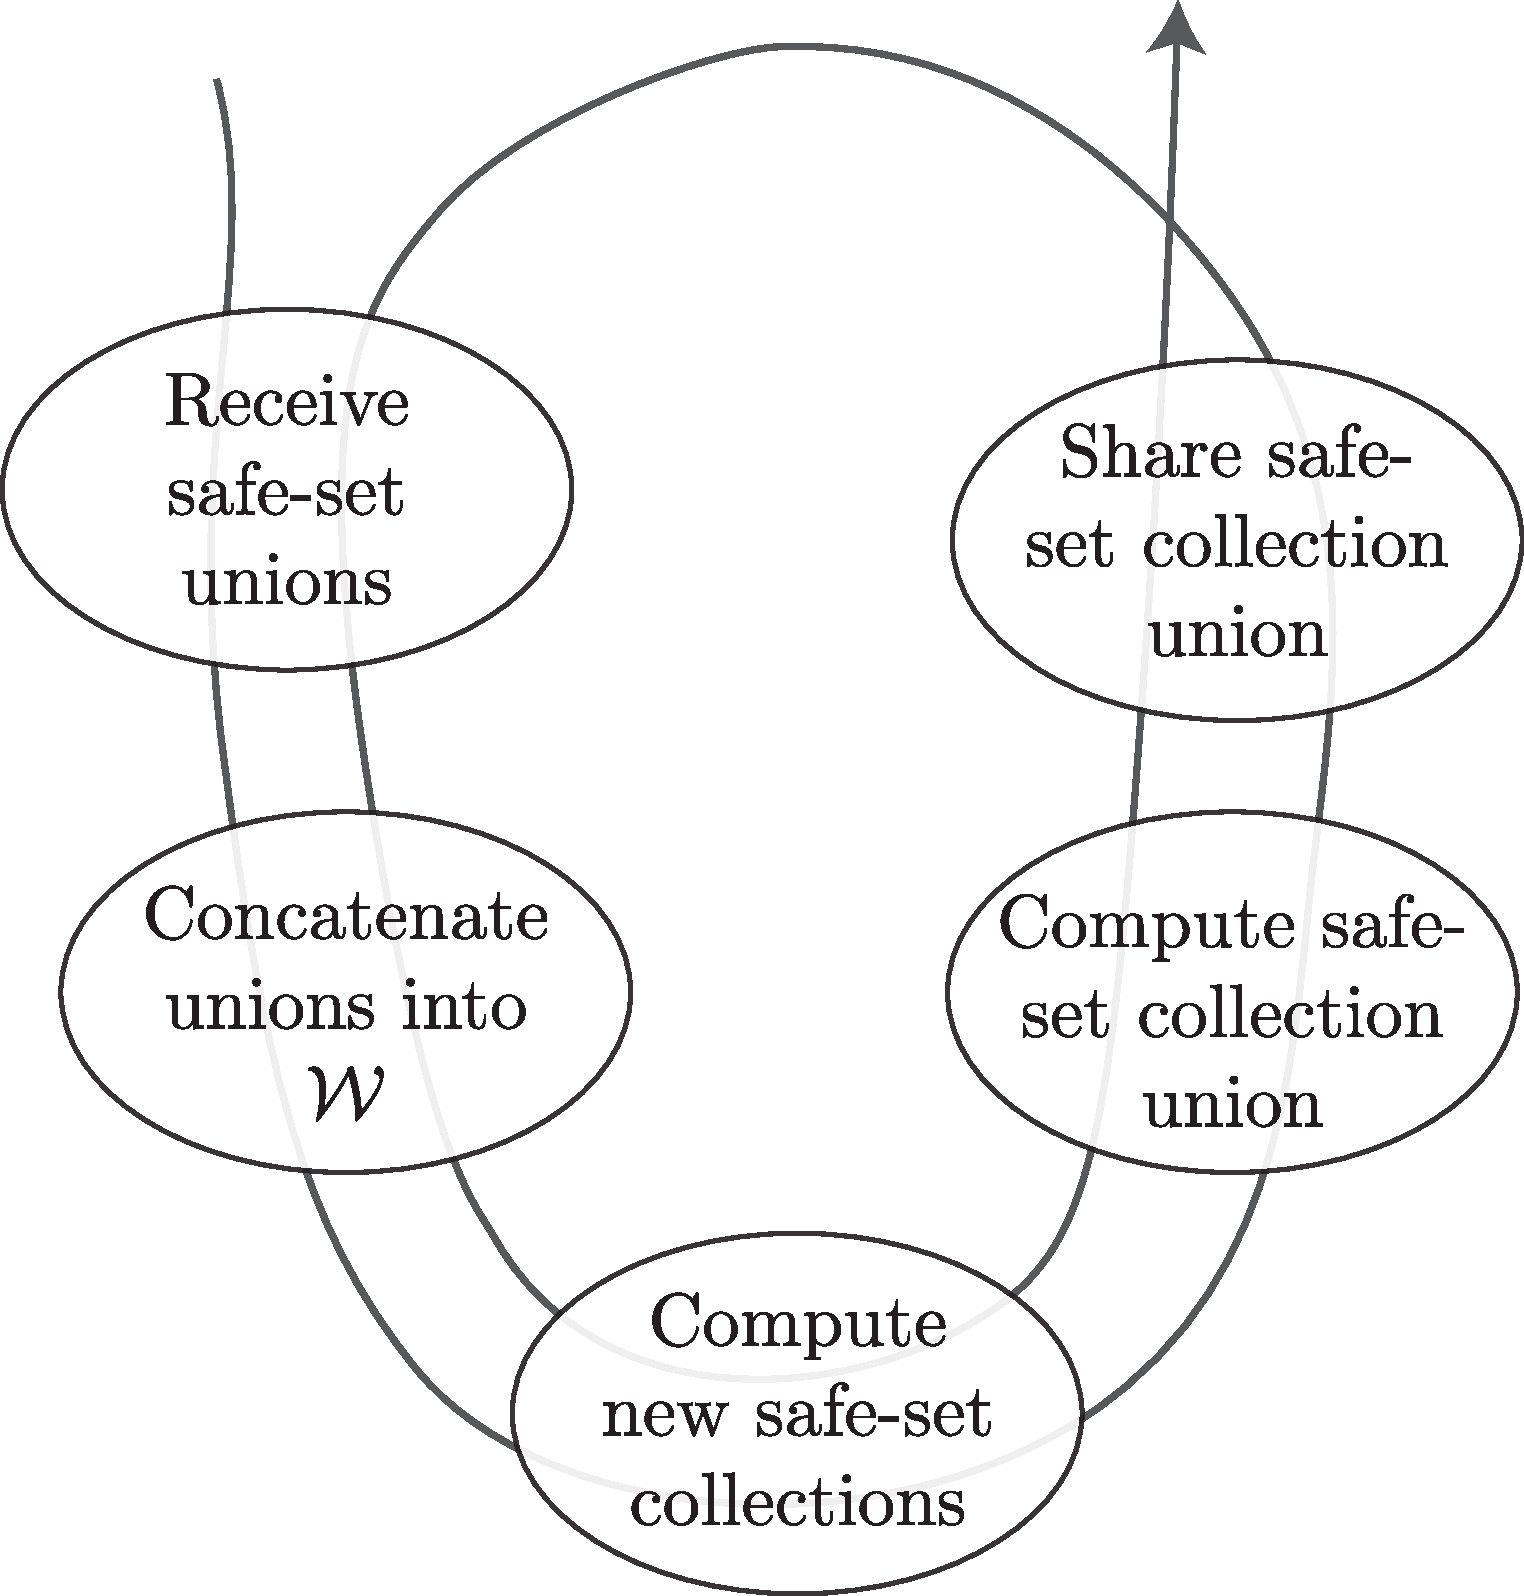
\includegraphics[width=0.75\columnwidth]{./figures/alg2_diag}
	\caption{Illustration of one iteration of \autoref{alg:safe_sets} from the perspective of a single agent. The algorithm is initialized with safe-set unions of $\underline{0}$ (see line 3 of \autoref{alg:safe_sets}). The algorithm continues until running this loop does not change any of the agents' safe set collection (line 17 of \autoref{alg:safe_sets})}
\end{figure}
\autoref{alg:node_safe_sets} is an important tool but requires that the safe-sets of the other block-rows are already known. As mentioned previously, there is a circular dependency where the neighboring safe-sets depend on the local safe-sets which, using \autoref{alg:node_safe_sets}, depends on the neighboring safe-sets. This circular dependency is addressed in \autoref{alg:safe_sets}. Starting from an initial, trivial guess for feasible, safe-set collections, the algorithm first generates safe-sets that are too large and infeasible and then safe-sets that are small but feasible. This process is repeated until a convergence criteria is met. Critically, the algorithm can be parallelized along the different block-rows. As block-rows are added, the computational complexity grows at a near linear rate as opposed to the exponential rate of the centralized case. Furthermore, as shown in the following lemma, the algorithm produces a feasible collection of safe-sets after each complete iteration. This allows the user to terminate after any complete iteration and produce valid results. 
\begin{algorithm}[t]
\caption{Distributed safe-set collection for system in \autoref{eq:agent_notation}}\label{alg:safe_sets}
\begin{algorithmic}[1]
\Procedure {SystemSafeSets}{$\agents$}
\State $\Omega^0\gets\{\{\underline{0}\}_{n\in\idxset{\gnumnodes[\agentidx]}}\}_{\agentidx\in\idxset{\numagents}}$
\State $\Phi^0\gets\{\underline{0}\}_{\agentidx\in\idxset{\numagents}}$
\State $k\gets0$
\Repeat
	\ParFor{each agent, $\agentidx\in\idxset{\numagents}$}
		\State $\wcon[\modeidx]^\agentidx\gets\prod_{\tilde{\agentidx}\in\idxset{\numagents}\setminus \agentidx}\Phi^{k}_{\tilde\agentidx}$ for all $\modeidx\in\idxset{\nummodes[\agentidx]}$
		\State $\Omega^{k+0.5}_{\agentidx}\gets\Call{AgentSafeSets}{\modes[\agentidx]}$
		\State $\Phi^{k+0.5}_{\agentidx}\gets\Call{ConHull}{\cup_{n\in\idxset{\gnumnodes[{\agentidx}]}}\Omega^{k+0.5}_{({\agentidx},n)}}$
	\EndParFor
	\ParFor{each agent, $\agentidx\in\idxset{\numagents}$}
		\State $\wcon[\modeidx]^\agentidx\gets\prod_{\tilde{\agentidx}\in\idxset{\numagents}\setminus \agentidx}\Phi^{k+0.5}_{\tilde\agentidx}$ for all $\modeidx\in\idxset{\nummodes[\agentidx]}$
		\State $\Omega^{k+1}_{\agentidx}\gets\Call{AgentSafeSets}{\modes[\agentidx]}$
		\State $\Phi^{k+1}_{\agentidx}\gets\Call{ConHull}{\cup_{n\in\idxset{\gnumnodes[{\agentidx}]}}\Omega^{k+1}_{({\agentidx},n)}}$
	\EndParFor
	\State $k\gets k+1$
\Until{$\Omega_{(\agentidx)}^k=\Omega_{(\agentidx)}^{k-1}\ \forall\ \agentidx\in\idxset{\agentidx}$}

\State $\safesets\gets\Omega^k$
\EndProcedure
\end{algorithmic}
\end{algorithm}
\begin{lemma}
For systems taking the form of \autoref{eq:sys} split into block rows as in \autoref{eq:block-row-dyn}, algorithm $\Call{SystemSafeSets}{\agents}$ produces a valid safe-set collection for every $k\in\int\rgeq{0}$. 
\end{lemma}
\begin{proof}
This holds trivially for $\Omega^0$. The following induction steps complete the proof.
\begin{enumerate}
	\item Assume $\Omega^k$ is valid under disturbance constraints $\Phi^k$.
	\item By Lemma 1, $\Omega^k\subseteq\Omega^{k+0.5}$.
	\item By Lemma 2, $\Phi^k\subseteq\Phi^{k+0.5}$ implies that $\Omega^{k+1}\subseteq\Omega^{k+0.5}$.
	\item Since $\Omega^{k+1}$ is valid for $\Phi^{k+0.5}$, it will also be valid for $\Phi^{k+1}$ since $\Phi^{k+1}\subseteq\Phi^{k+0.5}$.
\end{enumerate}
\end{proof}